\chapter[PDE and BL]{PDE and Boundary Layers}
\paragraph{Example:} Flame front propagation\footnote{J. Keener ``Principles of Applied Mathematics'' (1988), pp. 530-533}.
\begin{itemize}
	\item The independent variables are $\tau $ (time) and $\xi$ (1-D space)
	\item The temperature $\theta (\xi,\tau)$ and gas (fuel) concentration $y(\xi,\tau)$
	\item The Zeldovich number $\epsilon^{-1}\gg 1$ ($\epsilon \approx 0.1$) and Lewis number $L=D_T/D_Y$ which is the ratio of the heat diffusivity to the gas diffusivity
\end{itemize}
The scaled equations for this model read
\begin{align*}
	\frac{\pd \theta}{\pd \tau} &= \underbrace{\frac{\pd^2 \theta}{\pd \xi^2}}_\text{heat diffusion} +\underbrace{ \frac{1}{\epsilon^2} y f(\theta)}_\text{heat generated} \\
	\frac{\pd y}{\pd \tau} &= \underbrace{L^{-1} \frac{\pd^2 y}{\pd \xi^2}}_\text{gas diffusion} -  \underbrace{ \frac{1}{\epsilon^2} y f(\theta)}_\text{reaction consumes $y$}
\end{align*} 
where the reaction rate (from Arrhenius law) is
\begin{gather*}
	f(\theta) = \exp \left[\frac{\theta - 1}{\epsilon} \frac{1}{1+ \gamma (\theta-1)}\right]
\end{gather*}
Here $\theta$ has been normalized by the temperature at which the gas ignites, i.e. $\theta \in [0,1]$. So the curve of $f(\theta)$ vs. $\theta$ is essentially 0 upto a thin $O(\epsilon)$ neighborhood near the ignition temperature of 1, at which point it shoots to its maximum reaction rate.
\begin{figure}[!h]
	\centering
	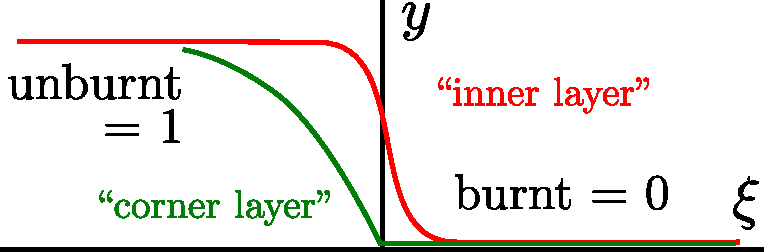
\includegraphics[width=0.6\textwidth]{./plots/pdf/burning-front-gas.pdf}\\ \vspace{5mm}
	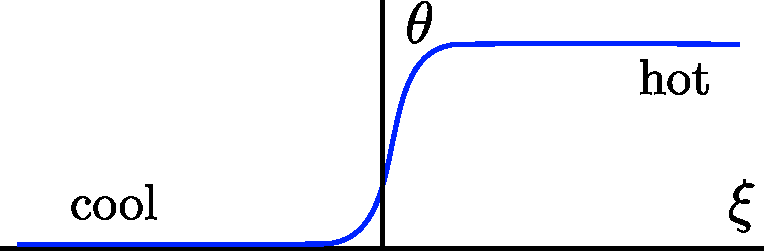
\includegraphics[width=0.6\textwidth]{./plots/pdf/burning-front-temp.pdf}
	\caption{(Top) Gas concentration $y$ as a function of space $\xi$ at a fixed time. (Bot) The corresponding temperature $\theta$ profile. }
	\label{fig:wk26}
\end{figure}
Intuitively, we expect the flame to propagate as a travelling wave of burning. We are especially interested in the wave speed (along with the profiles of gas concentration and temperature). Now was $\epsilon \rightarrow 0^+$, we expect something \underline{sharp} at the flame front (see Fig. \ref{fig:wk26}). However, it is not clear if the gas concentration $y$ should, in the buring zone, have an \emph{inner layer} (rapid change in $y$) or a \emph{corner layer} (rapid change in its derivative). These are naturally resolved in the course of our treatment. \\\\
Since we are interested in a travelling wave (to the left), we move into a co-moving frame with the transformation
\begin{gather*}
	s = v \tau + \xi, \qquad v >0
\end{gather*}
The advantage of this method is that it converts the PDE to an ODE; the value of $v$ is to be determined. Assume 
\begin{gather*}
	\theta = \theta(s) \qquad y = y(s)
\end{gather*}
i.e. the waves maintain their shapes and propagate leftwards. Using chain-rule to note
\begin{align*}
	\frac{\pd \theta}{\pd \tau} &= \frac{\pd \theta}{\pd s} \frac{\pd s}{\pd \tau } = v \theta_s \\
	\frac{\pd \theta}{\pd \xi} &= \frac{\pd \theta}{\pd s} \frac{\pd s}{\pd \xi } = \theta_s
\end{align*}
the PDEs become
\begin{align*}
	v \theta_s &= \theta_{ss} + \frac{1}{\epsilon^2} y f(\theta) \\
	v y_s &= L^{-1} y_{ss} - \frac{1}{\epsilon^2} y f(\theta)
\end{align*}
The above are a set of nonlinear ODEs with the (intuitively derived) BCs
\begin{align*}
	y(\infty) = 0, \qquad y(-\infty) = 1 \\
	\theta(\infty) = 1, \qquad \theta(-\infty) = 0
\end{align*} 
The hope is that the correct choice of the unknown velocity $v$ helps determine the BCs correctly. Define $s=0$ as the position of the wavefront and there should be some kind of internal layer near $s=0$.\\\\
\paragraph{Outer solns:} On the left, assume $\theta<1$ (it seems implausible that $\theta$ gets hotter ahead of the flame). For this $f(\theta)$ is a TST and no reaction is happening (flame has not arrived yet). With this
\begin{equation}\label{eqn:wk26-zero-rxnrate}
	\begin{split}
	v \theta_s &= \theta_{ss}\\
	v y_s &= L^{-1} y_{ss} 
	\end{split}
\end{equation}
which is simple uncoupled diffusion. Let us introduce
\begin{align*}
	\theta &= \theta_0 + \epsilon \theta_1 + \dots \\
	y &= y_0 + \epsilon y_1 + \dots \\
	v &= v_0 + \epsilon v_1 + \dots  
\end{align*}
With this the $O(1)$ equations are
\begin{align*}
	v_0 \theta_0' &= \theta''_0\\
	v_0 y_0' &= L^{-1} y''_0
\end{align*}
where the notation $f' = \md f / \md s$ has been introduced. We can straightforwardly integrate to write
\begin{gather*}
	\theta_0(s) = a \me^{v_0s} + c_1, \qquad \theta_0(-\infty) = 0 \\
	\implies \theta_0(s) = a \me^{v_0 s}
\end{gather*}
This is exponential decay from $s=0$ as $s$ goes left. Similarly solving for the gas concentration with $y_0(-\infty)=1$ we see
\begin{gather*}
	y_0(s) = 1 - b \me^{L v_0 s} 
\end{gather*}
On the right, $s>0$, $y=0$ and $\theta=1$ -- therefore $f(\theta)=0$. This also yields the equation set \ref{eqn:wk26-zero-rxnrate}. Like before, an exponential term arises and these must be set to zero to prevent blow-up as $s \rightarrow \infty$. This yields the solution
\begin{gather*}
	\theta_0(s) = 1, \qquad y_0(s) = 0
\end{gather*}
If the solutions to the left and right are to match at $s=0$, it must be that $a=1$ and $b=1$. Altogether, for $s \leq 0$
\begin{align*}
	\theta_0(s) &= \me^{v_0s} \\
	y_0(s) &= 1 - \me^{L v_0 s} 
\end{align*}
\begin{itemize}
	\item The pictures are suggesting a corner layer at $s=0$
	\item $\theta_0 < 1$ for $s<0$ as we hoped (self-consistent) 
	\item $v$ is not determined yet:  the $f(\theta)$ was missing.
\end{itemize}
So we need to get into the {\bf inner region} where the burning is happening. To find $v_0$ we need to match more carefully near $s=0$. The term $y f(\theta)/\epsilon^2$ becomes significant near $s=0$. Now $\theta$ behaves linearly\footnote{$\me^{v_0s} \approx v_0s + \dots $} with $s$ in the immediate left neighborhood of $s=0$. Since we are interested in {\color{red} [check argument]}
\begin{align*}
	\theta \approx v_0s \sim 1 - \epsilon 
\end{align*}
(such that $f(\theta)\sim O(1)$ and not TST) we are interested in $s \leq O(\epsilon)$. \\\\
The form of $f(\theta)$ thereby motivate the strected variables
\begin{gather}\label{eqn:wk26-cl-vars}
	\eta = \frac{s}{\epsilon} \qquad \theta - 1 = \epsilon \phi \qquad y = \epsilon u
\end{gather}
\begin{figure}[!h]
	\centering
	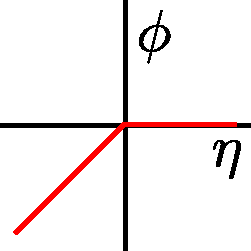
\includegraphics[width=0.2\textwidth]{./plots/pdf/burning-front-phi.pdf} \qquad 
	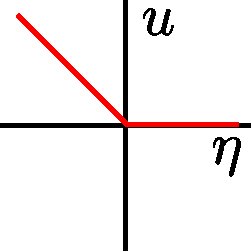
\includegraphics[width=0.2\textwidth]{./plots/pdf/burning-front-u.pdf}
	\caption{The corner layer variables using the scalings in eqns. \ref{eqn:wk26-cl-vars} and Fig. \ref{fig:wk26}.}
	\label{fig:wk26-phi-u}
\end{figure}
Intuitively, the burning zone would look like a sharply peaked Gaussian: to the left and right the reaction rate is almost zero. With these transformations the derivatives are
\begin{align*}
	\frac{\md y}{\md s} &= \frac{\md}{\md (\epsilon \eta)} (\epsilon u ) = \frac{\md u}{\md \eta} \\
	\frac{\md^2 y}{\md s^2} &= \frac{\md}{\md (\eta \epsilon)} \frac{\md u}{\md \eta} = \frac{1}{\epsilon} \frac{\md^2 u}{\md \eta^2}
\end{align*}
implying
\begin{flalign*}
	\phi'' - \epsilon v \phi' + uf(1+\epsilon\phi)=0 \\
	L^{-1}u'' - \epsilon v u' - uf(1+\epsilon\phi)=0
\end{flalign*}
and
\begin{align*}
	f(1+ \epsilon \phi) &= \me^{\phi/ (1+ \gamma \epsilon \phi) }= \me^{(\phi_0 + \dots )(1 - \gamma \epsilon \phi_0 + )} \\
	&\sim \me^{\phi_0 + O(\epsilon)} \approx \me^{\phi_0} [1 + O(\epsilon)]
\end{align*}
So at $O(1)$ we get
\begin{align}
	\phi_0'' + u_0 \me^{\phi_0} = 0 \label{eqn:wk26-cl-phi}\\
	L^{-1}u_0'' - u_0 \me^{\phi_0} = 0 \label{eqn:wk26-cl-u}
\end{align}
Adding eqns. \ref{eqn:wk26-cl-phi} and \ref{eqn:wk26-cl-u} we can get rid of the nonlinear term to write
\begin{align*}
	\phi_0'' + L^{-1} u_0'' &= 0 \\
	\implies \phi_0 + L^{-1}u_0 &= c_1 \eta + c_2
\end{align*}
With the help of Fig. \ref{fig:wk26}, and noting that $u,\phi$ are just scaled versions of $y, \theta $ (latter offset by one), we conclude that as $\eta \rightarrow \infty$, both $u,\phi \rightarrow 0$. Therefore, since
\begin{align*}
	\phi_0 + L^{-1}u_0 \rightarrow 0 \\
	\phi_0' + L^{-1}u_0' \rightarrow 0
\end{align*}  
it must be that $c_1=c_2=0$ yielding
\begin{gather}
	\phi_0 = -L^{-1}u_0
\end{gather}
With this insight we can write eqn. \ref{eqn:wk26-cl-phi} as
\begin{gather*}
	\phi_0'' - L \phi_0 \me^{\phi_0} = 0
\end{gather*}
{\bf NB.} This is of the form $\ddot x = -kx$ except that the force depends on the displacement in some non-linear way. The trick to find the constant of motion for such sytems is to multiply through with $\phi_0'$ and integrate\footnote{Such as in deriving the energy for the Duffing oscillator (eqn. \ref{eqn:wk22-duffing-energy}).}:
\begin{gather*}
	\frac{\md}{\md \eta } \left[\frac{1}{2} \phi_0'^2 - Lg(\phi_0) \right] = 0
\end{gather*}
such that
\begin{align*}
	g(\phi_0) &= \int   \phi_0 \phi_0' \me^{\phi_0} \md \eta = \int \phi_0 \frac{\md \me^{\phi_0}}{\md \eta}  \md \eta \\
	&= \phi_0 \me^{\phi_0} - \int \phi_0' \me^{\phi_0} \md \eta \\
	&= (\phi_0-1) \me^{\phi_0} + c
\end{align*}
Therefore 
\begin{gather*}
	\frac{1}{2} \phi_0'^2 - L(\phi_0 - 1)\me^{\phi_0} = c
\end{gather*}
Using the fact that as $\eta \rightarrow \infty$, $\phi_0 \rightarrow 0$ 
\begin{align*}
	-\frac{1}{2}(0)^2 -L(-1)\me^0 = c \qquad \implies c=L
\end{align*}
We arrive at the implicit equation for $\phi_0 (\eta)$. What's remaining is to match the slope $\phi_0'$ at $\eta \rightarrow -\infty$ to the incoming slope from the outer solution on the left. The figure helps us understand that $\phi_0(\eta) \rightarrow -\infty$ as $\eta \rightarrow -\infty$. Therefore
\begin{gather*}
\frac{1}{2} \phi_0'^2 - \underbrace{L(\phi_0 - 1)\me^{\phi_0}}_\text{TST} = L \\
\implies \phi_0'(-\infty) = \pm \sqrt{2L}
\end{gather*}
We keep the positive root as is once again seen from the figure. Matching slopes
\begin{align*}
	\left. \frac{\md}{\md s} (\me^{v_0 s})\right|_{s=0^-} &= \left. \frac{\md \phi}{\md \eta}\right|_{\eta = -\infty} \\
	\implies v_0 &= \sqrt{2L}
\end{align*}










